%!TEX root = Main.tex
\documentclass[Main]{subfiles}

\begin{document}

\section{Contribution} % (fold)
\label{sec:contribution}

	The contribution from this mini-project consists of an implementation and test of the DFTSP.
	The implementation builds upon the FTSP implementation already available for TinyOS\cite{FTSPImplementationTinyOS:Online}.
	\subsection{Implementation} % (fold)
	\label{sub:implementation}

		\subsubsection{DFTSP Mote} % (fold)
		\label{sub:dftsp_mote}
			The DFTSP has been implemented on Crossbow Telosb motes\cite{TelosBDatasheet:Online} running the TinyOS\cite{TinyOS:Online} operating system.

			Kan du lave nesc documentation Ivan? 
			command: nesdoc -o doc -target=telosb DFTSPAppC.nc

		tempSensorRef \cite{tempSensorDatasheet}
		% subsubsection dftsp_mote (end)
		
		
		\subsubsection{Broadcaster Motes} % (fold)
		\label{sub:broadcaster_mote}
		
		% subsubsection broadcaster_mote (end)
	

		
		\subsubsection{Serial Java Application} % (fold)
		\label{sub:serial_java_application}
		
		% subsection serial_java_application (end)

	% subsection implementation (end)

	\subsection{Test Setup} % (fold)
	\label{sub:test_setup}

		\begin{figure}[H]
			\centering
			\includegraphics[width=\linewidth]{TestSetup.jpg}
			\caption{Test Setup}
			\label{fig:TestSetup}
		\end{figure}
	
	% subsection test_setup (end)

	\subsection{Test Results} % (fold)
	\label{sub:test_results}

		\subsubsection{Stable Environment} % (fold)
		\label{sub:stable_environment}
		
		% subsubsection stable_environment (end)

		\subsubsection{Unstable Environment} % (fold)
		\label{sub:unstable_environment}
			
			\begin{figure}[H]
				\centering
				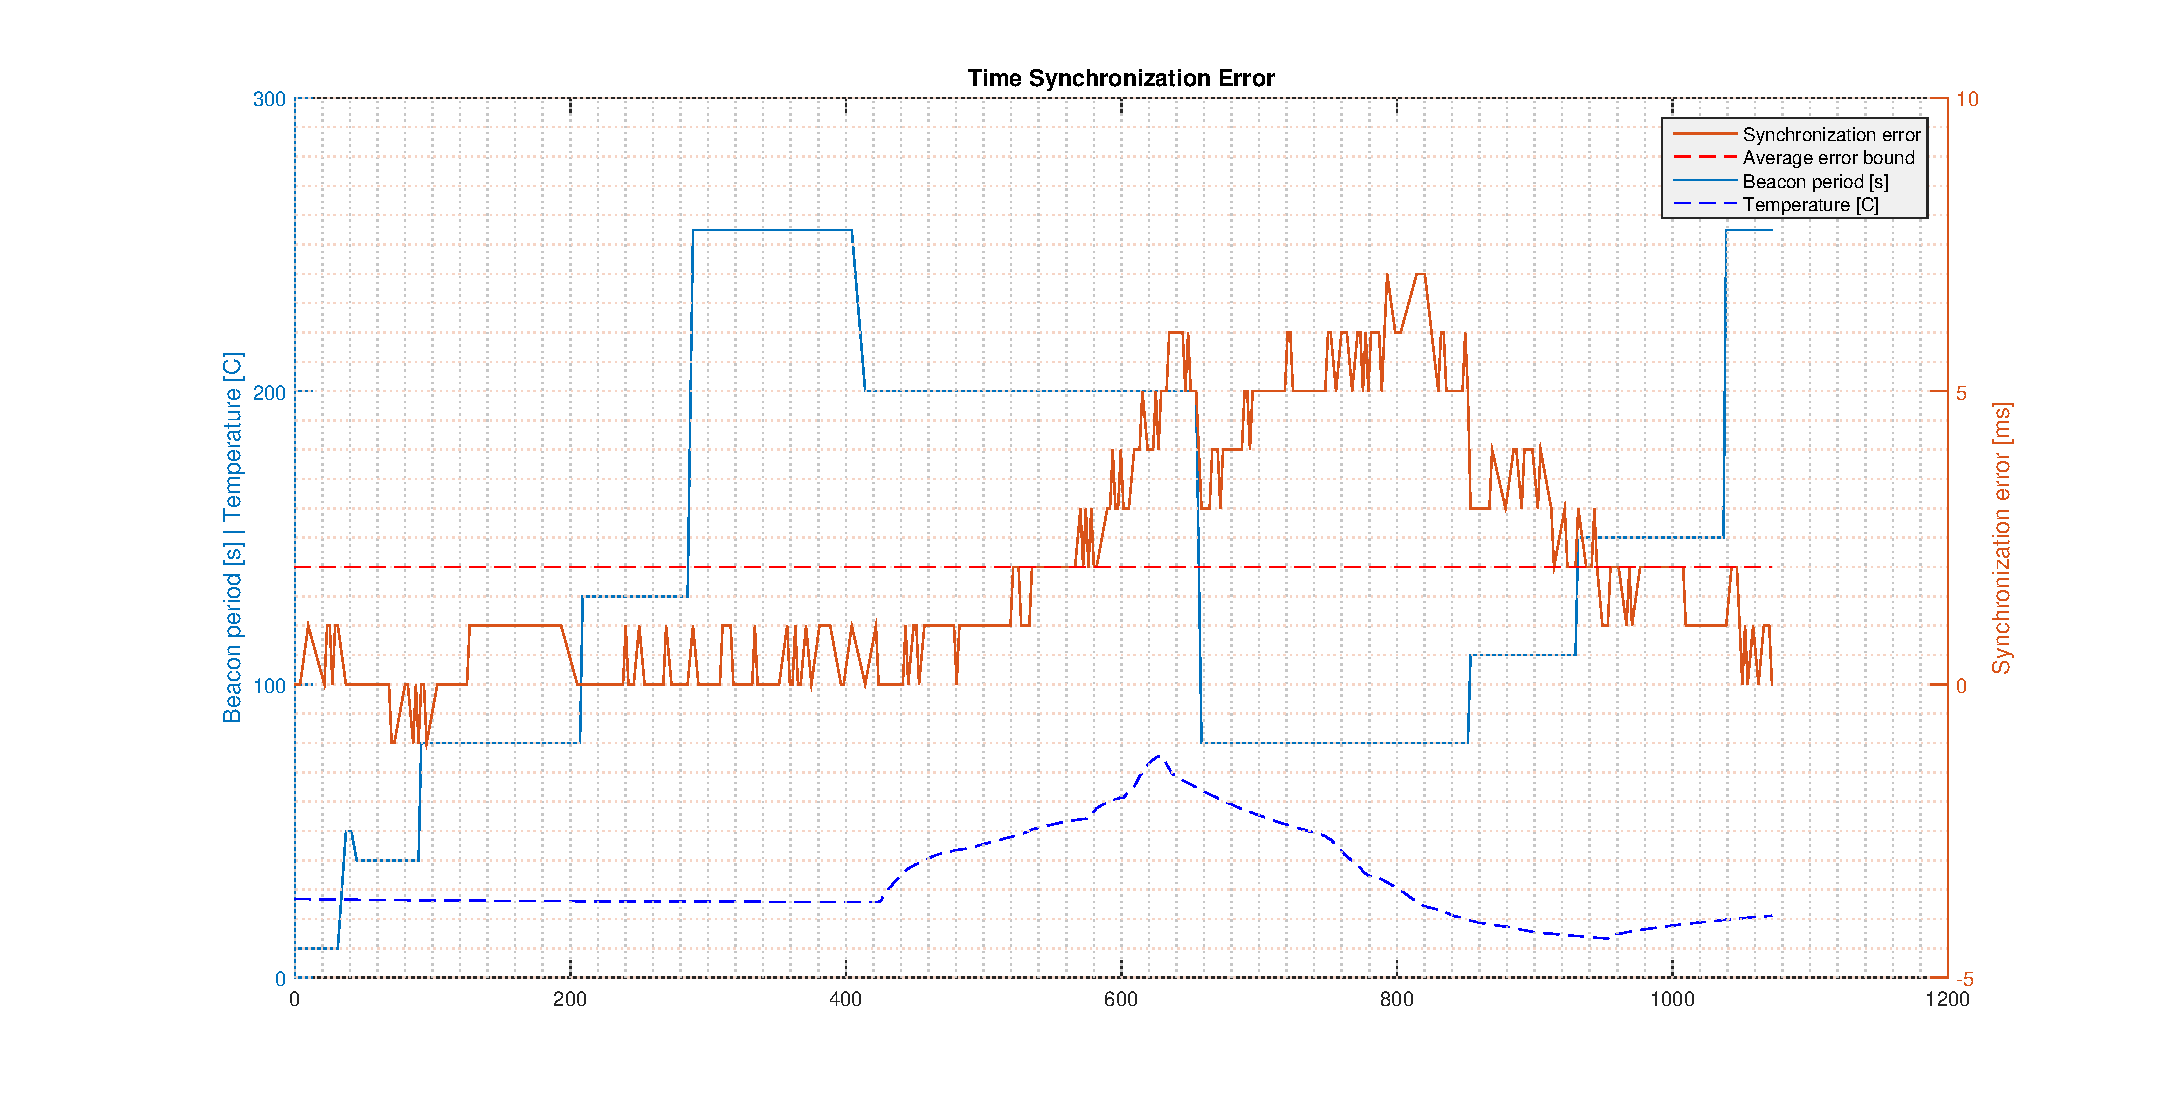
\includegraphics[width=\linewidth]{Synchronization.eps}
				\caption{Time Synchronization Error}
				\label{fig:Synchronization}
			\end{figure}

		% subsubsection unstable_environment (end)
	
	% subsection test_results (end)

% section contribution (end)

\end{document}
